\chapter{Server Side}
\begin{figure}[!ht]
  \centering
  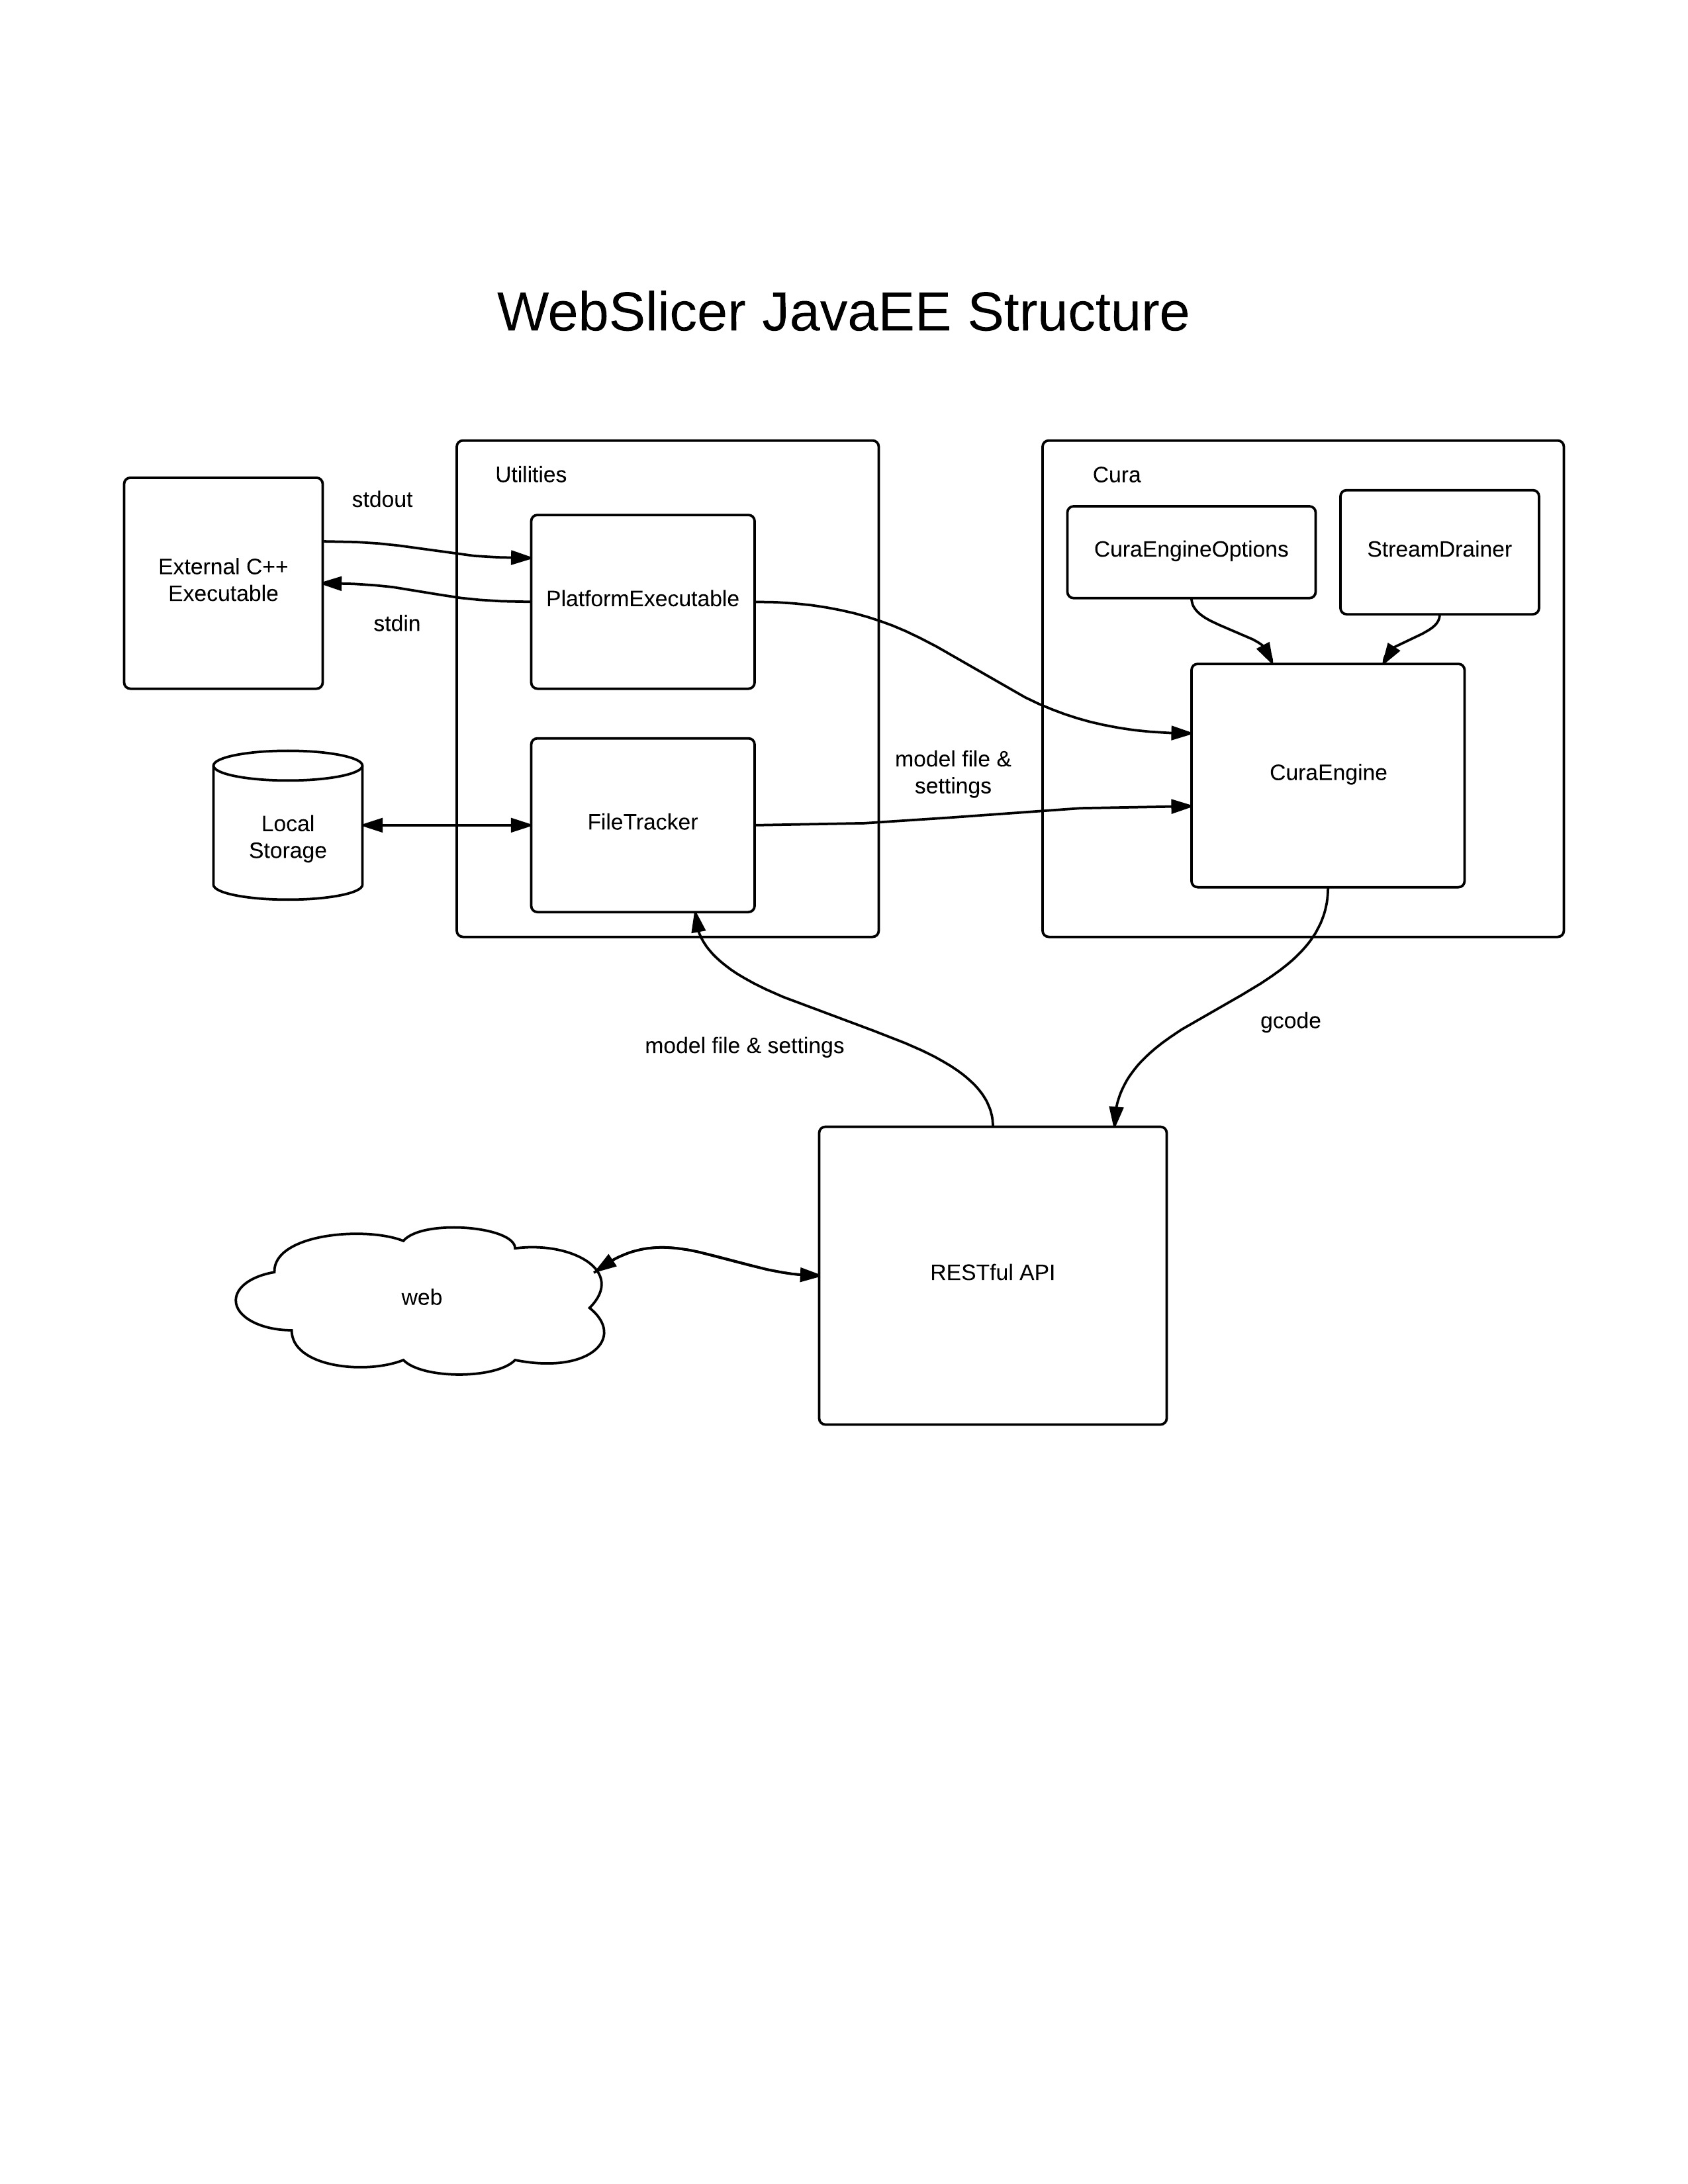
\includegraphics[width=\linewidth]{Server-Side-Structure}
  \caption{The structure of the server side of WebSlicer}
  \label{fig:server-side-structure}
\end{figure}

\section{JavaEE 7}
% talk about why its awesome and how i structured my code.
% give enough background to exalain what is needed
% maven archetype stuff
\paragraph{}
The majority of the server side of WebSlicer was written in JavaEE, the structure for which is shown in Figure \ref{fig:server-side-structure}.
JavaEE was the optimal choice for this application as it allowed for the easiest deployment and was also the easiest to scale.
To further simplify the process Maven was also used.
Maven is a build tool for Java and has support for deploying complex applications such as those in JavaEE.
This meant that when a build was completed it was automatically deployed and ready for testing.

\section{ProcessBuilder}
% ignore CuraEngine and talk only about how ProcessBuilder works with diagrams
\paragraph{}
At the core of the server side application is a core executable called CuraEngine. 
It is the main executable which is compiled from the open source slicing platform Cura which is written in C++. 
This presented a problem as all of my server side code is written in Java. 
ProcessBuilder was the solution to this problem as it is capable of redirecting the input and output streams of a local executable process into my Java server application.

%include code listing of where the executable would be called. keep it consise.

\section{CuraEngine Integration}
% how it works with ProcessBuilder

\section{REST API}
% my REST API and the reason that I structured it the way I did
% make a table which shows my API and its mapping then explain each function
\paragraph{}
\begin{center}
    \begin{tabular}{ | l | l | l | p{5cm} |}
    \hline
    Day & Min Temp & Max Temp & Summary \\ \hline
    Monday & 11C & 22C & A clear day with lots of sunshine.  
    However, the strong breeze will bring down the temperatures. \\ \hline
    Tuesday & 9C & 19C & Cloudy with rain, across many northern regions. Clear spells 
    across most of Scotland and Northern Ireland, 
    but rain reaching the far northwest. \\ \hline
    Wednesday & 10C & 21C & Rain will still linger for the morning. 
    Conditions will improve by early afternoon and continue 
    throughout the evening. \\
    \hline
    \end{tabular}
\end{center}


\section{Key Challenges}
\subsection{ProcessBuilder Deadlock}
\begin{figure}[!ht]
  \centering
  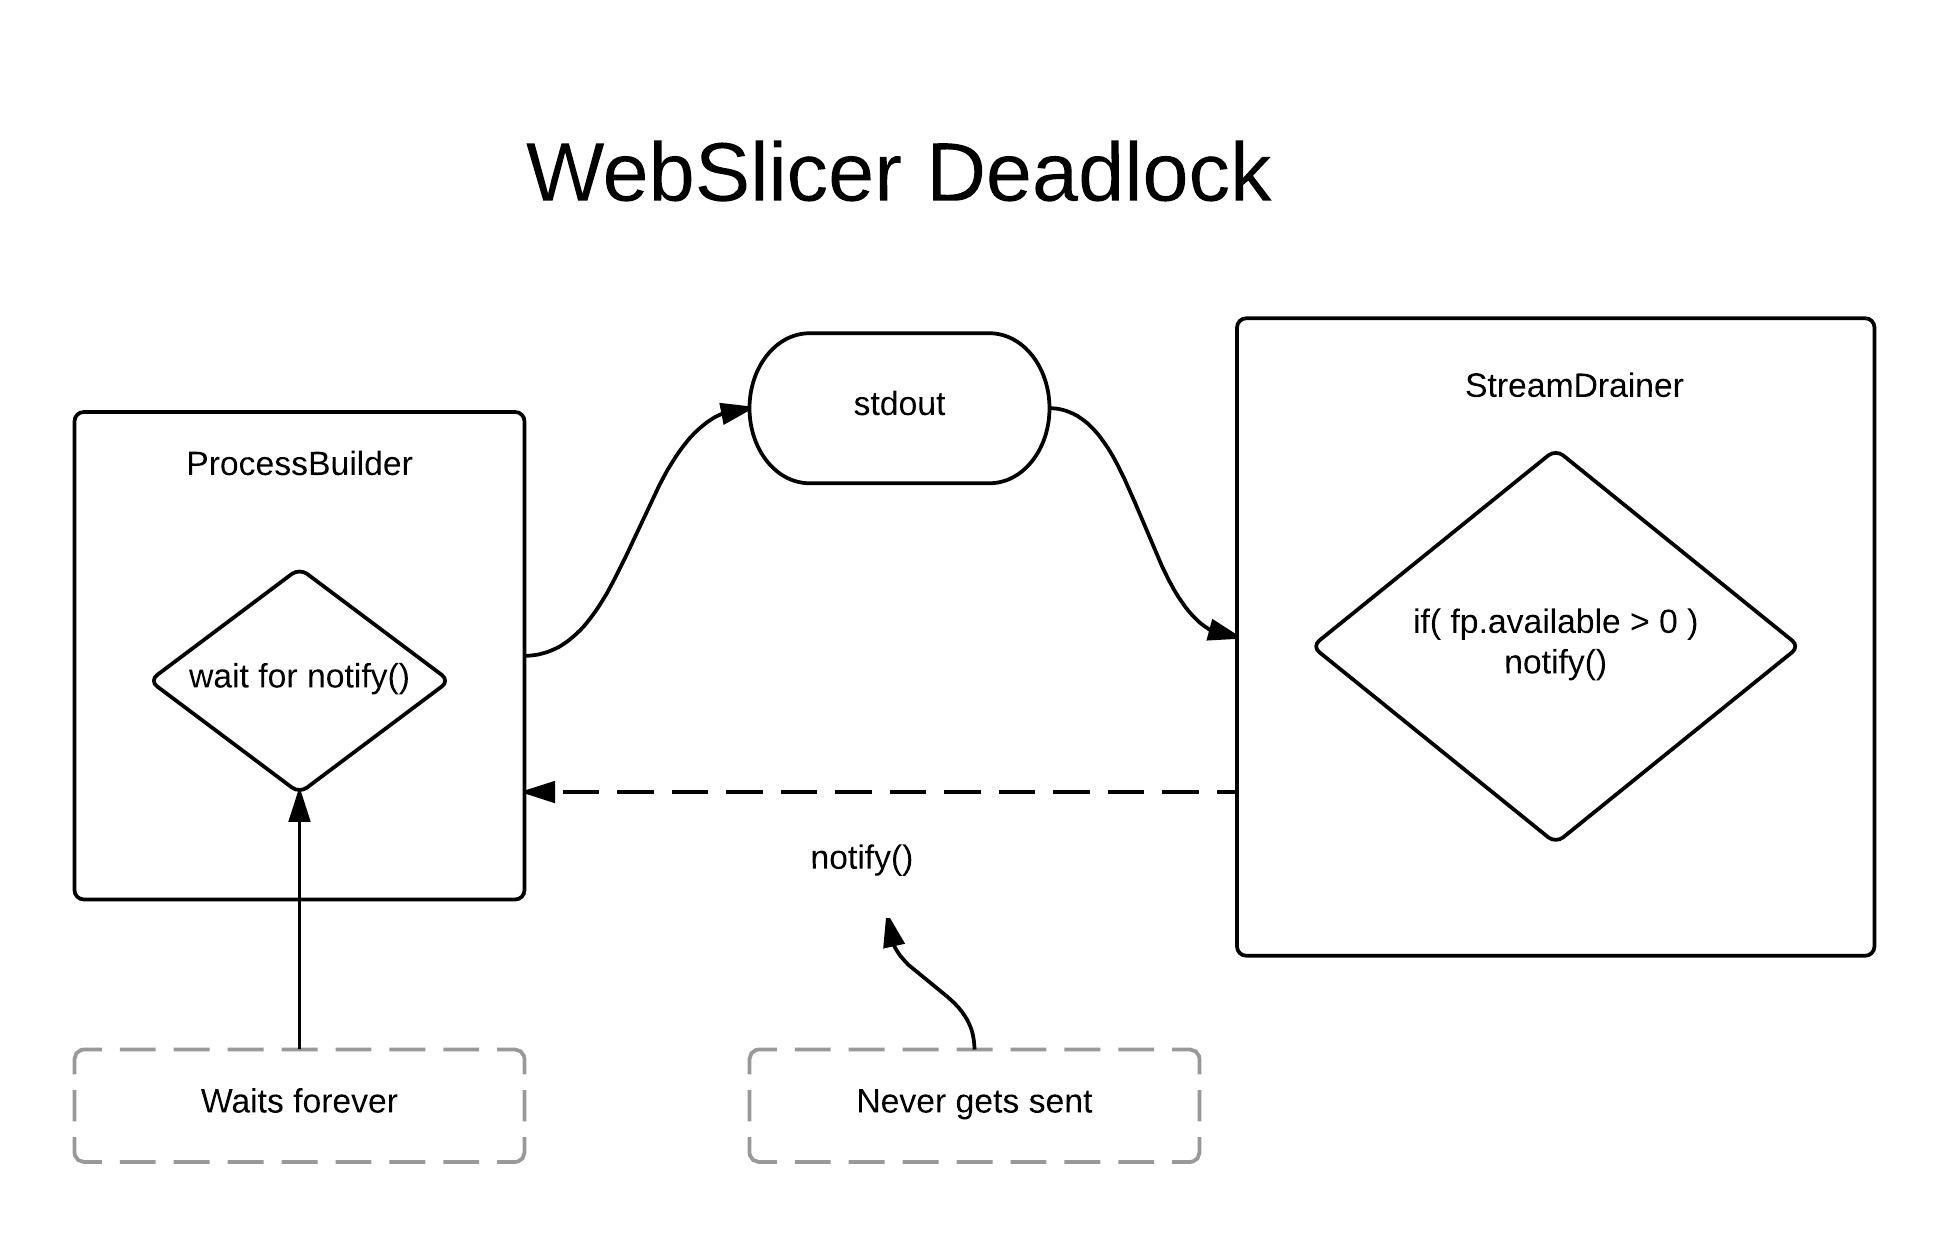
\includegraphics[width=\linewidth]{Deadlock-Diagram}
  \caption{Diagram of a deadlock issue that took weeks to resolve}
  \label{fig:deadlock-diagram}
\end{figure}
\paragraph{}
One of the biggest bugs encountered while developing this project was a thread deadlock issue. 
The server side code uses java’s ProcessBuilder which builds a system native call to an executable and then pipes the input and output into the input and output pipes of java’s stdio as shown in Figure \ref{fig:deadlock-diagram}.
This works very well for small platform executable’s with limited I/O but can become problematic when complex native calls such as the curaengine are used.

\paragraph{}
ProcessBuilder does its normal writes to stdout and the drainer just pipes them into a file. 
However the drainer has to wait for a file pointer using the fp.available() function. 
This is a non blocking function which only estimates the buffer size that it has for the file. 
The check for file pointer availablity was checking if this function returned something greater than 0 as an estimate before notifying the ProcessBuilder that it was ready. 
However the buffer size would often start as zero before allocation and as this check was not part of a loop it would stay stuck forever as the notify was missed.

\paragraph{}
This problem was solved by using the correct blocking file pointer available check. 
Occasionally the buffer size was larger than 0 and the application ran fine but with some models it would consistently fail as the buffer had not been allocated yet.
This solution is seemingly obvious yet this solution still took many days to find and correct as the application did not fail consistently.

\subsection{FileTracker Revamp}
\paragraph{}
The first iteration of FileTracker was a bit crude and not well planned out. 
It tracked two hashmaps, one for model files and the other for settings files with no mind for the client who actually needed to have access to those files. 
This worked fine for testing but had many pitfalls including the inablility to reuse files that already existed. 
As soon as the client died those files were lost which is a major inefficiency.

\paragraph{}
The fdmprinter.json file within the unique client folder is symbolically linked to the fdmprinter.json file within common. 
The CuraEngine executable requires that all of the settings files rest within the same directory when preforming a slice. 
This is somewhat problematic with the potential of having this file copied for many clients. 
Thus, symbolically linking the file to the rescue.

\paragraph{}
The output.gcode and settings.json files are dynamically overwritten for every iteration so their existence here is merely to please CuraEngine as it requires these files as arguments when preforming a slice. 
The user has no grasp of these files and is only able to access their content through the web interface which parses in and out of files.

%listing
\begin{lstlisting}[language=html, style=thesiscode, label={lst:file-structure}, caption=WebSlicer's underlying file structure supported by FileTracker.]
webslicer/
- b1a2a69e-5893-4d7c-aa1f-d639fa3b4ed1/
  - fdmprinter.json -> /tmp/webslicer/common/fdmprinter.json
  - models/
     - balanced_die_version_2.stl
     - raldrich_planetary.stl
  - output.gcode
  - settings.json
- common/
  - fdmprinter.json
  - presets/
    - prusa_i3.json
    - ultimaker2.json
\end{lstlisting}

\section{Future Improvements}
\paragraph{}
Currently FileTracker does not take advantage of the presets within the common/presets/ folder as described by Listing \ref{lst:file-structure}. 
These files contain the default settings for the corresponding printer which right now are only the ultimaker2 and a basic configuration of a prusa i3 variant. 
Optimally, the user would select from one of these starting presets and then modify and save their own.
This would allow users an optimal starting point and lowering the amount of starting knowledge and increasing the usability of WebSlicer.

\paragraph{}
This new file structure also allowed for an easy client index. 
In the future the unique folder ID will become the client's identification number which will be tied to their login. 
Additionally, simplifying the login process with googles oauth 2.0 system was also planned.

\section{Issues \& Known Bugs}
\paragraph{}
Currently there is no way for the server to import existing user files into its structure.
This means that when the server is restarted for any reason that the entire supporting file structure with all user files is lost.
Resolving this is just a matter of writing an initial import function that indexes all of the existing files.
It was left out of the initial version due to time constraints.
